\chapter{Prompt gamma detection}\label{chap::2}

\vfill

\minitoc

\newpage

\glsresetall

Ion beam therapy is rapidly emerging as a valuable cancer treatment technique and a superior alternative to photon radiotherapy for specific clinical indications. The narrow dose peak at the end of the ion range allows for targeted delivery of high dose to the tumor while sparing healthy surrounding tissues. However, since such a treatment technique is highly sensitive to dose prediction and delivery uncertainties, online range monitoring solutions are necessary. Over- and under-shooting effects potentially lead to severe damages to healthy tissues and/or treatment inefficiency, and thus have to be controlled in real-time. The research effort in this field mainly focuses on the non-invasive detection of primary by-products of beam-tissue nuclear interactions: photons from electron-positron annihilation and prompt gammas are most extensively studied for this purpose. 
The research work presented in this thesis focus on the development of gamma cameras for the detection of prompt gamma rays to tackle the challenge of real-time range monitoring during particle therapy treatments. In this chapter, after a brief introduction of the photon interaction channels in matter, the main topic of the thesis will be addressed by discussing the present developed techniques to obtain information about the ion range with prompt gamma ray detection. Finally, the state-of-the-art of gamma detectors employed for this purpose is sketched.

\section{Photon detection}


\subsection{Photon interactions in matter}

In penetrating an absorbing medium, photons may experience various interactions with the atoms of the medium, involving either the nuclei or the orbital electrons. The interactions with nuclei may be direct photon-nucleus collisions or interactions between the photon and the electrostatic field of the nucleus (pair production). On the other hand, the photon-orbital electron interactions can involve either loosely bound electrons (binding energy $E_B$ small in comparison with the photon energy $h\nu$ - $E_B \ll h\nu$) or tightly bound electrons (binding energy comparable to, or slightly smaller than the photon energy - $E_B  \lesssim h\nu$). 
All these processes are characterized by a partial or complete energy transfer of the gamma-ray photon, and two different outcomes are possible:
\begin{itemize}
\item Photon disappears (i.e. is completely absorbed) and its energy is transferred to light charged particles (electron and positrons);
\item Photon is scattered and two results are possible:
	\begin{itemize}
		\item the resulting photon has the same energy as the incident photon and no light charged particle is released in the interaction;
		\item the resulting scattered photon has a lower energy than the incident photon and the energy excess is transferred to a light charged particle (electron).
	\end{itemize}
\end{itemize}

We focus here on the interaction channels which play an important role in radiation measurements: 
\begin{itemize}
\item photoelectric absorption;
\item Compton scattering;
\item pair production.
\end{itemize}

In case the photon interacts with an absorber \myMarginnote{Photoelectric absorption} atom and completely disappears by transferring all its energy to the target, the interaction mechanism is called photoelectric absorption. In the interaction an orbital electron  is ejected with kinetic energy $E_K$ corresponding to the difference between the incident photon energy $h\nu$ and the electron binding energy $E_B$, as reported in equation~\ref{chap2::eq::energyPhotoelectron}. The ejected orbital electron is generally referred to as \enquote{photoelectron}. A schematic view of the photoelectric absorption mechanism is shown in \figurename~\ref{chap2::fig::photoel_abs}.

\begin{equation}
E_K = h\nu - E_B
\label{chap2::eq::energyPhotoelectron}
\end{equation}

\begin{figure}[!htbp]
\centering
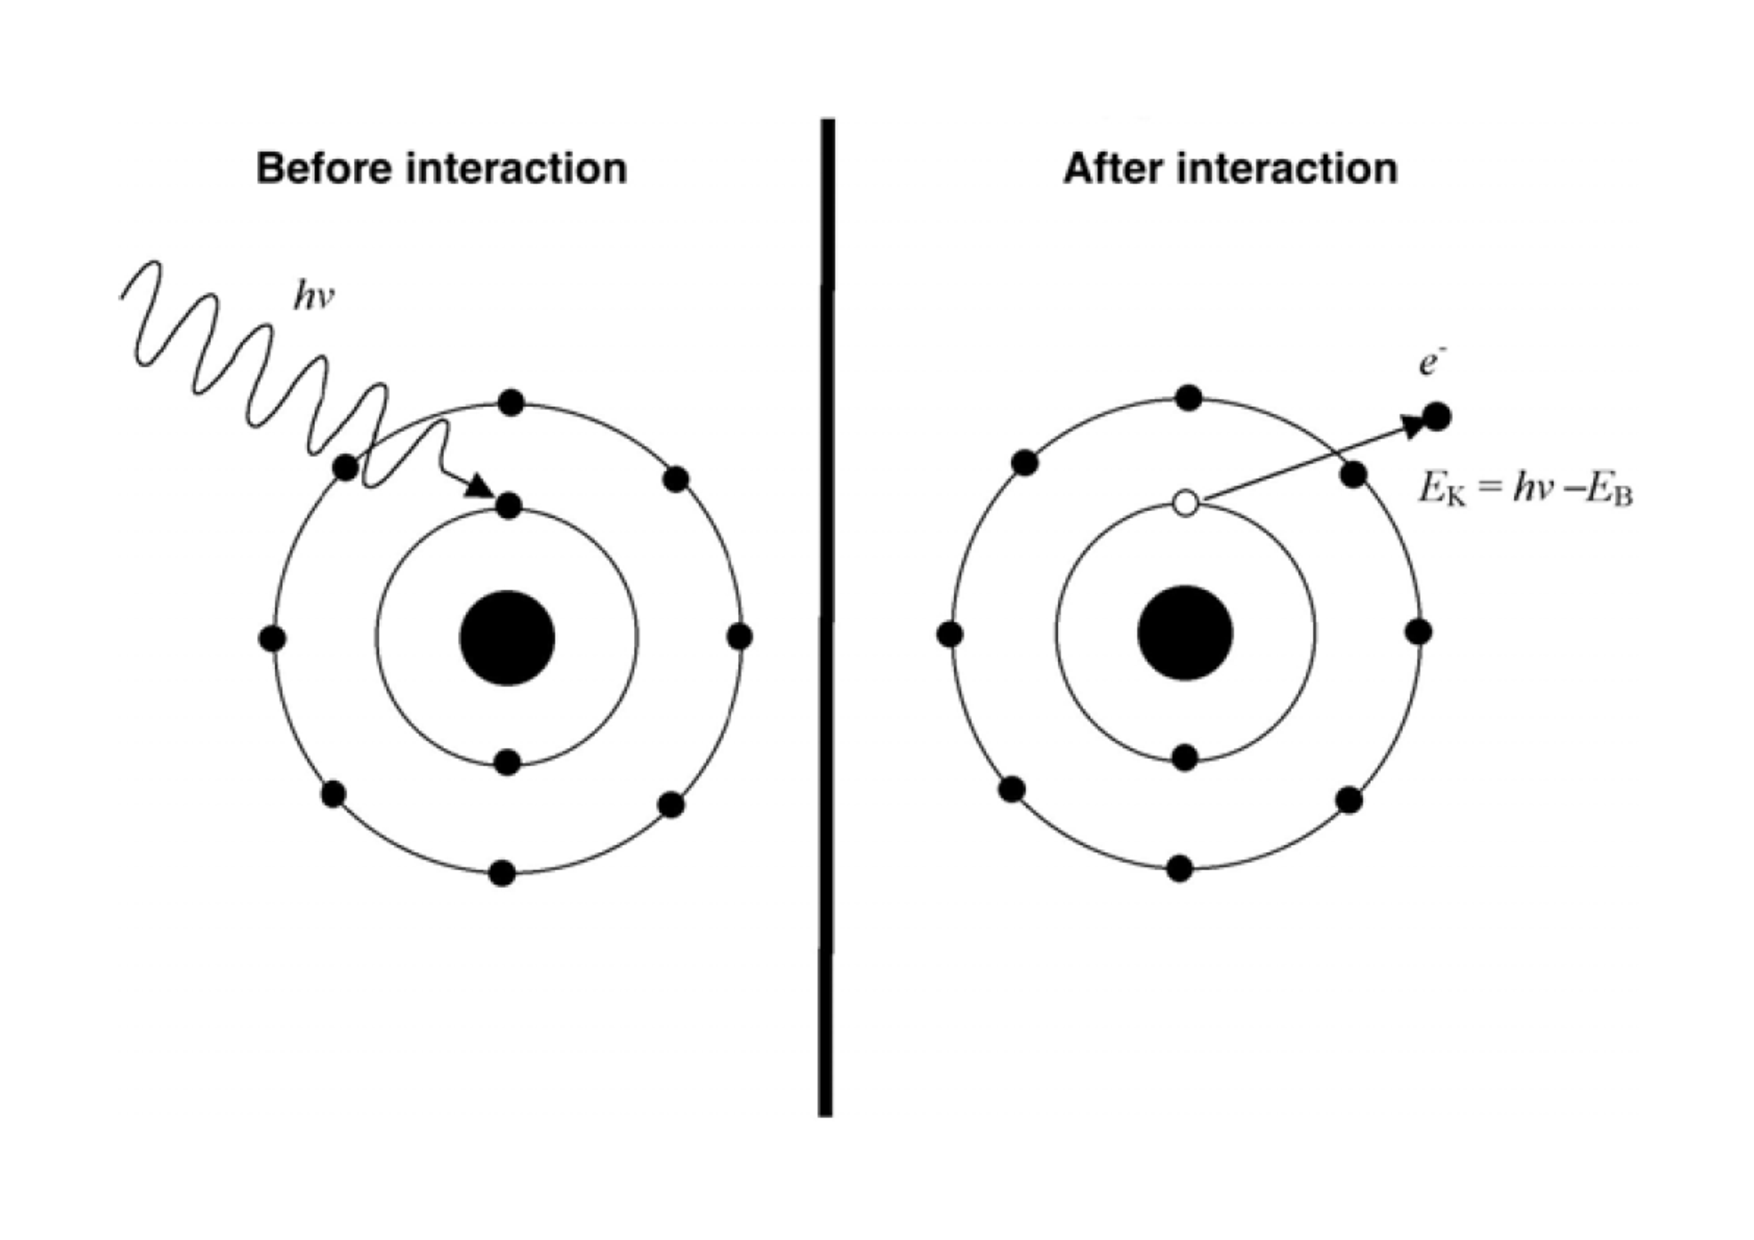
\includegraphics[width=0.8\textwidth]{03_GraphicFiles/chapter2_GammaCameras/photoelectric_abs.pdf}
\caption{Schematic diagram of the photoelectric effect. A photon with energy $h \nu$ interacts with a K-shell electron, which is ejected as photoelectron with kinetic energy $E_K$. In~\cite{Podgorsak2010}.}
\label{chap2::fig::photoel_abs}
\end{figure} 

The interaction is with the atom as a whole, and cannot take place with free electrons for conservation of energy and momentum constraints, although the whole photon energy is transferred to an atomic electron in one of the atom bound shells (tightly bound electron). Energy and momentum cannot be conserved simultaneously in a photon-free electron interaction: the momentum conservation requires a third object (the atom) involved in the interaction which must absorb the extra momentum. When the photon energy exceeds the K-shell binding energy of the absorber, about 80\% of all photoelectric absorption interactions occur with the K-shell electrons. If the energy transferred to the photoelectron is not below the binding energy threshold, it can be sufficient to raise it to a higher orbit, in a process of excitation. 
As a result of the photoelectric absorption, in addition to the ejected photoelectron, the absorber atom has a vacancy in one of its bound shells. This vacancy is quickly filled through capture of a free electron of the medium and/or rearrangement of electrons from other shells at higher energy level. Therefore, depending on the involved shells, one or more characteristics x-ray photons (fluorescent photons) may also be generated. Such photons are generally reabsorbed close to the original atom site through a further photoelectric absorption involving less tightly bound shells. In some fraction of the cases, the emission of an Auger electron may substitute for the characteristic x-ray in carrying away the atomic excitation energy. As the fluorescent photons, Auger electrons are generally reabsorbed very near the site of the original interaction.
The photoelectric process is the predominant mode of interaction for gamma rays of relatively low energy, and it is also enhanced for absorber materials of high atomic number Z. Even if a single analytic expression for the probability of photoelectric absorption over all ranges of photon energy $E_{\gamma}$ and Z, the probability ($\sigma_{PE}$)dependence on these two parameters can be approximated as shown in equation~\ref{chap2::eq::photoelProb}, where $n$ varies in the range [4,5] depending on the photon energy (4 for relatively low photon energies, 5 in the relativistic region)~\parencite{Knoll2000}.

\begin{equation}
\sigma_{PE} \varpropto \frac{Z^n}{E^{3.5}_{\gamma}} 
\label{chap2::eq::photoelProb}
\end{equation}  
 
In \figurename~\ref{chap2::fig::photonCrossSec} the cross section for the photoelectric absorption is compared to the one of the other photon interaction mechanisms for a copper absorber as a function of the photon energy. It exhibits a characteristic sawtooth structure in which the sharp discontinuities arise whenever the photon energy coincides with the binding energy of a particular electron shell. Except for the K shell, all other shells have a fine energy structure which reflect in the cross section curve.  

An interaction of a photon of energy $h\nu$ \myMarginnote{Compton scattering} with a loosely bound orbital electron of an absorber is called Compton scattering in honor of Arthur Compton who made the first measurements of photon-\enquote{free electron} scattering in 1923~\parencite{Compton1923}. Compton earned the Nobel prize for the discovery in 1927.  
In Compton scattering, the incoming gamma-ray photon is deflected through an angle $\theta$ with respect to its original direction, while transferring a portion of its energy to the electron, referred to as \enquote{recoil electron}. In theoretical studies of such an interaction mechanism, an assumption is made that the photon interacts with a free and stationary electron. As a result of the interaction, the photon, which had an initial energy $h\nu$, continue traveling in the new direction (angle $\theta$ with respect to the incident direction) with reduced energy $h\nu'$, and the recoil electron is ejected from the atom with a kinetic energy $E_K$ and a direction with an angle $\phi$ with respect the photon incident direction. A schematic view of the interaction is given in \figurename~\ref{chap2::fig::compton_principle}.
The expression that relates the energy transfer and the scattering angle for any given interaction can be derived by writing simultaneous equations for the conservation of energy and momentum. The obtained relationship is presented in equation~\ref{chap2::eq::Compton}, with the notation described above and $m_{0}c^2$ the rest-mass energy of the electron (511~keV). From the same calculation the kinetic energy of the recoil electron is also obtained from the expression in equation~\ref{chap2::eq::ComptonRecEnergy}.

\begin{equation}
h\nu' = \frac{h\nu}{1+\frac{h\nu}{m_{0}c^2}(1-\cos(\theta))}
\label{chap2::eq::Compton}
\end{equation} 

\begin{equation}
E_K = h\nu \frac{\frac{h\nu}{m_0c^2} (1-\cos(\theta))}{1+\frac{h\nu}{m_{0}c^2}(1-\cos(\theta))}
\label{chap2::eq::ComptonRecEnergy}
\end{equation} 

\begin{figure}[!htbp]
\centering
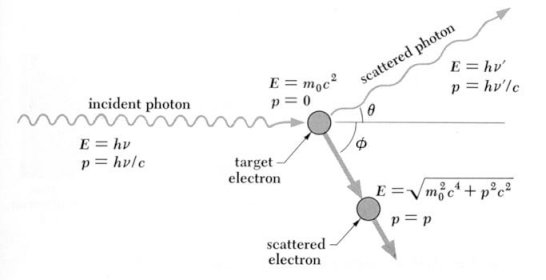
\includegraphics[width=0.8\textwidth]{03_GraphicFiles/chapter2_GammaCameras/ComptonPrinciple.jpg}
\caption{Schematic view of the Compton scattering principle. Image from https://universe-review.ca/R15-12-QFT10.htm.}
\label{chap2::fig::compton_principle}
\end{figure} 

From equation~\ref{chap2::eq::Compton} emerges how small scattering angles correspond to little energy transfers, and the other way around. In particular, for $\theta = 0$, no energy is transferred to the electron and the interaction becomes a classical Thomson scattering. For for $\theta > 0$ the energy of the scattered photon saturates at high values of the incident photon energy; the larger is the scattering angle, the lower is the saturation value of $h\nu'$ for $h\nu \lim \infty$
The relationship between the photon energy before and after the interaction is shown in \figurename~\ref{chap2::fig::ComptonEnergy} for various scattering angles $\theta$ between 0\textdegree (forward scattering) and $\pi$ (back-scattering.) 
The scattering angle $\theta$ and the recoil electron angle $\phi$ are related by equation~\ref{chap2::eq::ComptonAngles}.

\begin{equation}
\cot(\phi) = (1+\frac{h\nu}{m_{0}c^2})\tan\bigg(\frac{\theta}{2}\bigg)
\label{chap2::eq::ComptonAngles}
\end{equation} 

This relationship shows that for a given $\theta$, the higher is the incident photon energy $h\nu$, the smaller is the recoil electron angle $\phi$. In \figurename~\ref{chap2::fig::thetaphirel} the scattering and recoil angle dependence is plotted for different values of $\epsilon = h\nu / m_{0}c^2$.

\begin{figure}
\centering
\begin{subfigure}[t]{.49\textwidth}
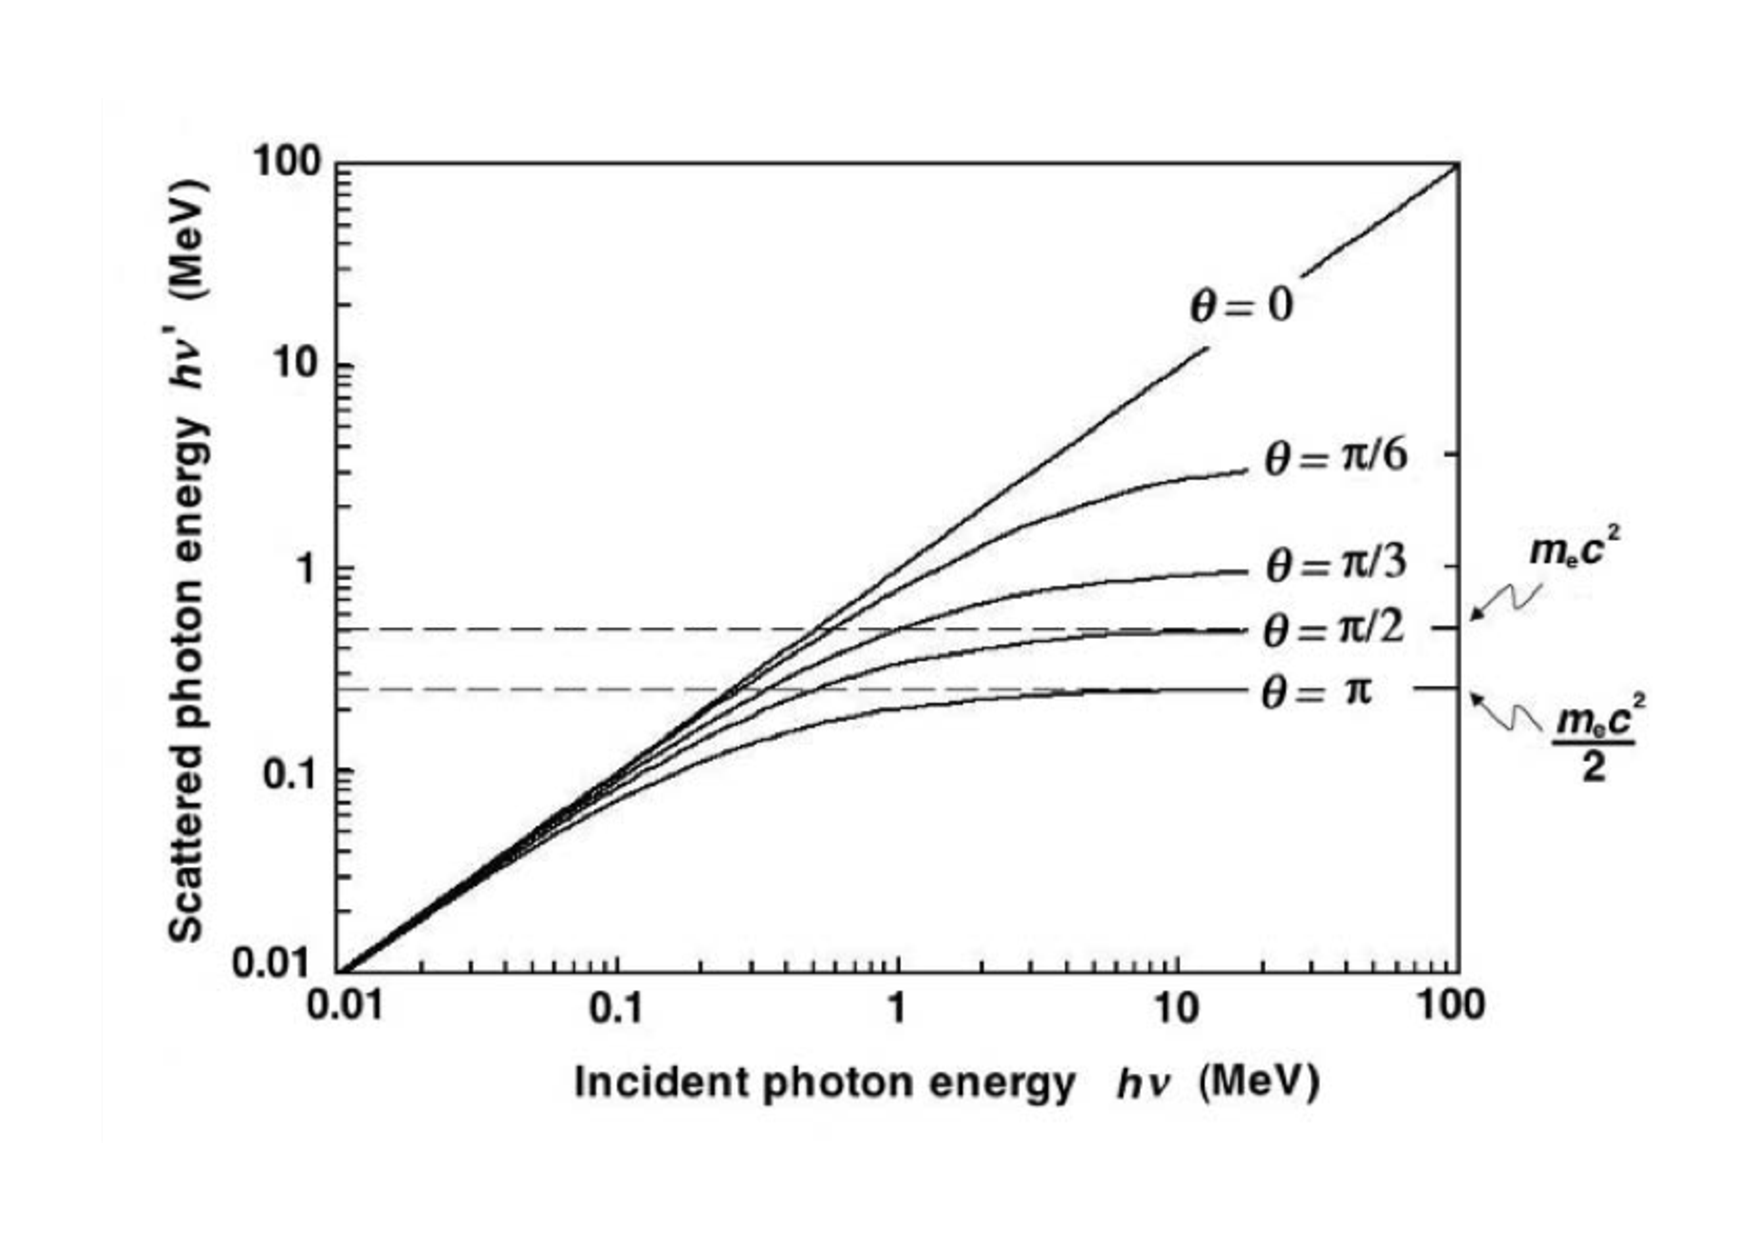
\includegraphics[width=1.1\linewidth]{03_GraphicFiles/chapter2_GammaCameras/ComptonEnergy.pdf}
\caption{Scattered photon energy against the incident photon energy for various Compton scattering angles in the range from 0\textdegree to $\pi$.}
\label{chap2::fig::ComptonEnergy}
\end{subfigure}
\begin{subfigure}[t]{.49\textwidth}
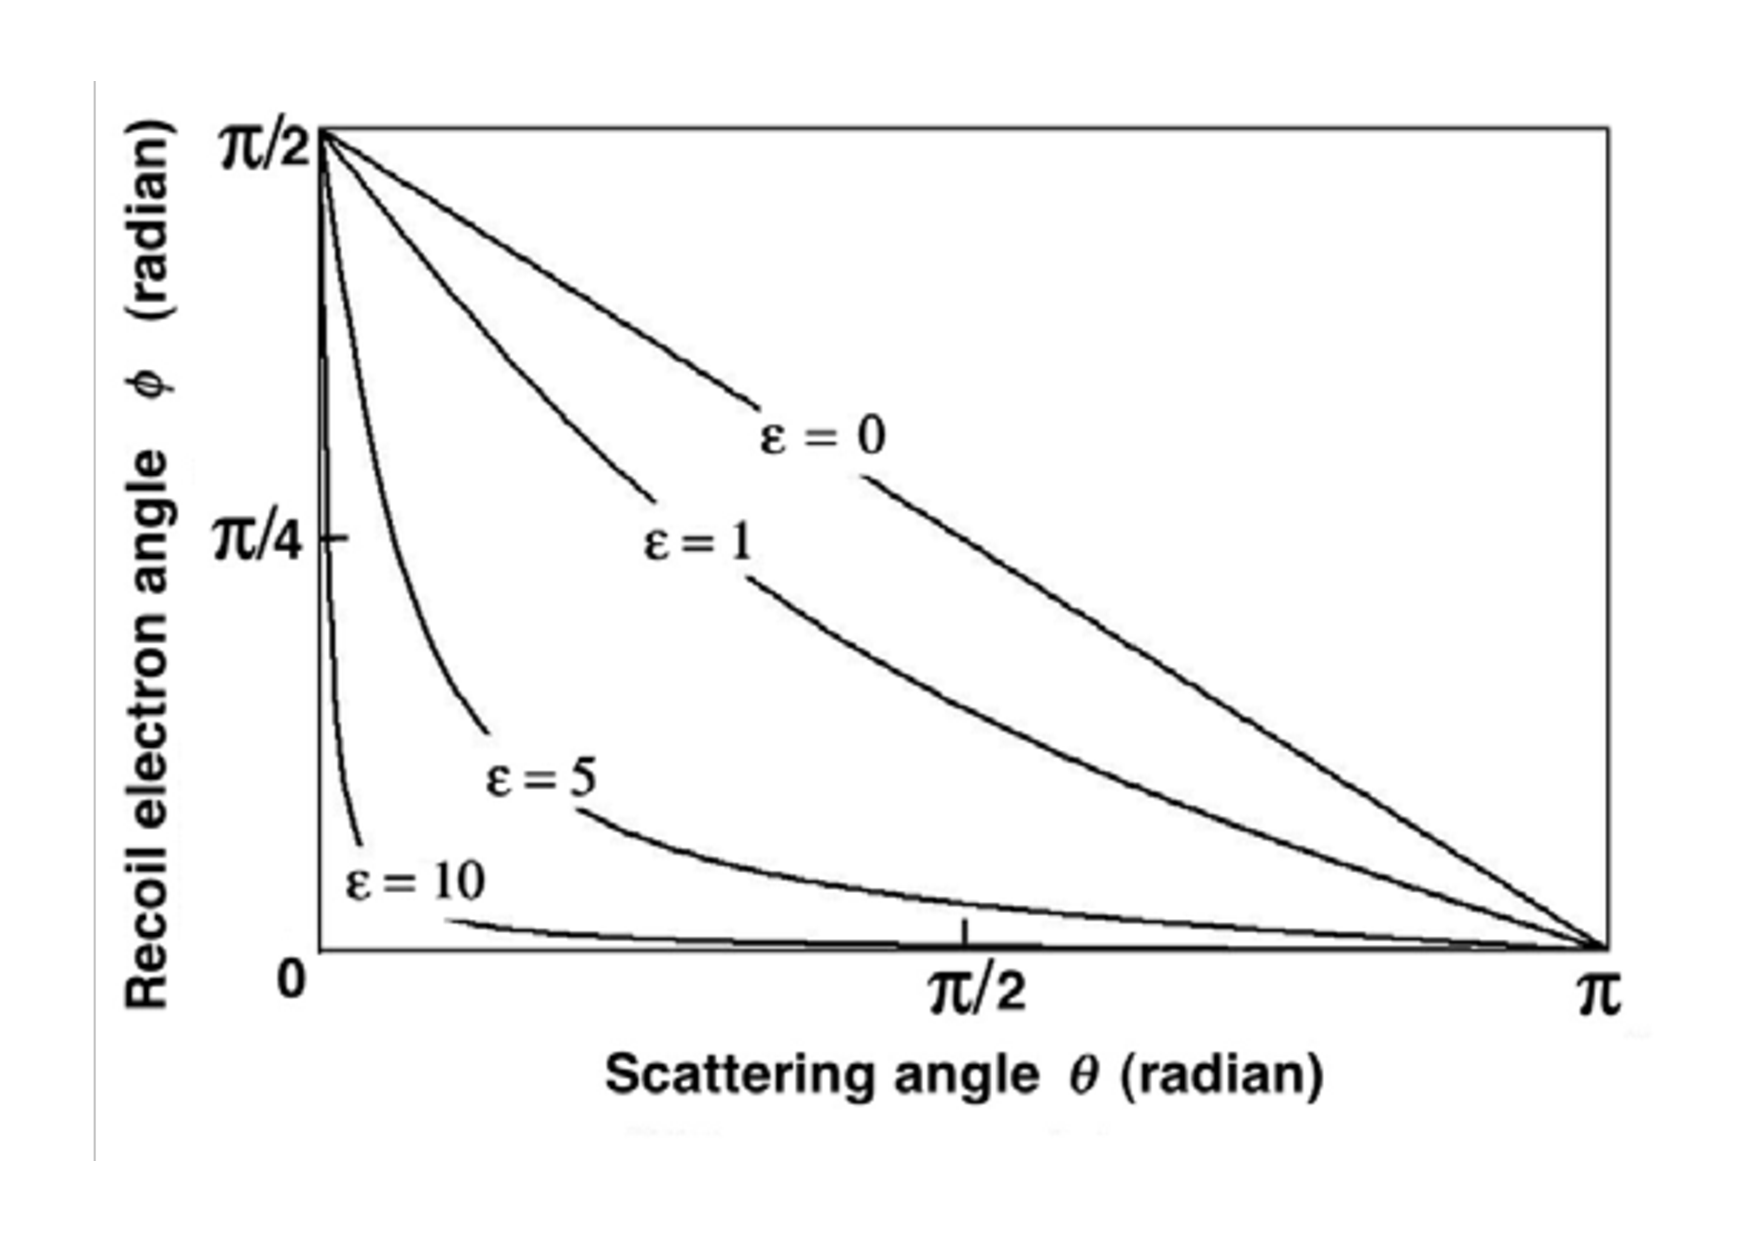
\includegraphics[width=1.1\linewidth]{03_GraphicFiles/chapter2_GammaCameras/scattRecoilAnglesCompton.pdf}
\caption{Relationship between the electron recoil electron $\phi$ and the photon Compton scattering angle $\theta$.}
\label{chap2::fig::thetaphirel}
\end{subfigure}
\caption{In~\cite{Podgorsak2010}}
\label{chap2::fig::ComptonAngular}
\end{figure}
   
The probability of Compton scattering per atom of the absorber depends on the number of electrons available as scattering targets and therefore linearly increases with the atomic number Z. In \figurename~\ref{chap2::fig::photonCrossSec} the probability energy dependence is shown for a copper target and compared to the other interaction channels probability. The differential cross section, or angular distribution of scattered gamma rays, is predicted by a formula derived by Oskar Klein and Yoshio Nishina in 1929, and reported in equation~\ref{chap2::eq::KleinNishina}~\parencite{Klein1929}.
 \begin{equation}
\frac{\mathrm{d}\sigma}{\mathrm{d}\Omega} = Zr_{e}\bigg(\frac{1}{1+\epsilon (1-\cos(\theta))}\bigg)^{2}\bigg( \frac{1+\cos^2(\theta)}{2} \bigg)\bigg(1+\frac{\epsilon^2(1-\cos(\theta))^2}{(1+\cos^2(\theta)[1+\epsilon(1-\cos(\theta))])} \bigg) 
\label{chap2::eq::KleinNishina}
\end{equation} 
where $r_{e}$ is the classical electron radius expressed in equation~\ref{chap1::eq::electronRad}. The distribution is shown graphically in \figurename~\ref{chap2::fig::ComptonAngCrossSection} and illustrates the strong tendency for forward scattering at high values of the gamma-ray energy. At low incident photon energies the probability for forward scattering and back-scattering are equal and twice as large as the probability for side scattering. As the incident photon energy increases, the scattering becomes increasingly more forward peaked and back-scattering rapidly diminishes.

\begin{figure}[!htbp]
\centering
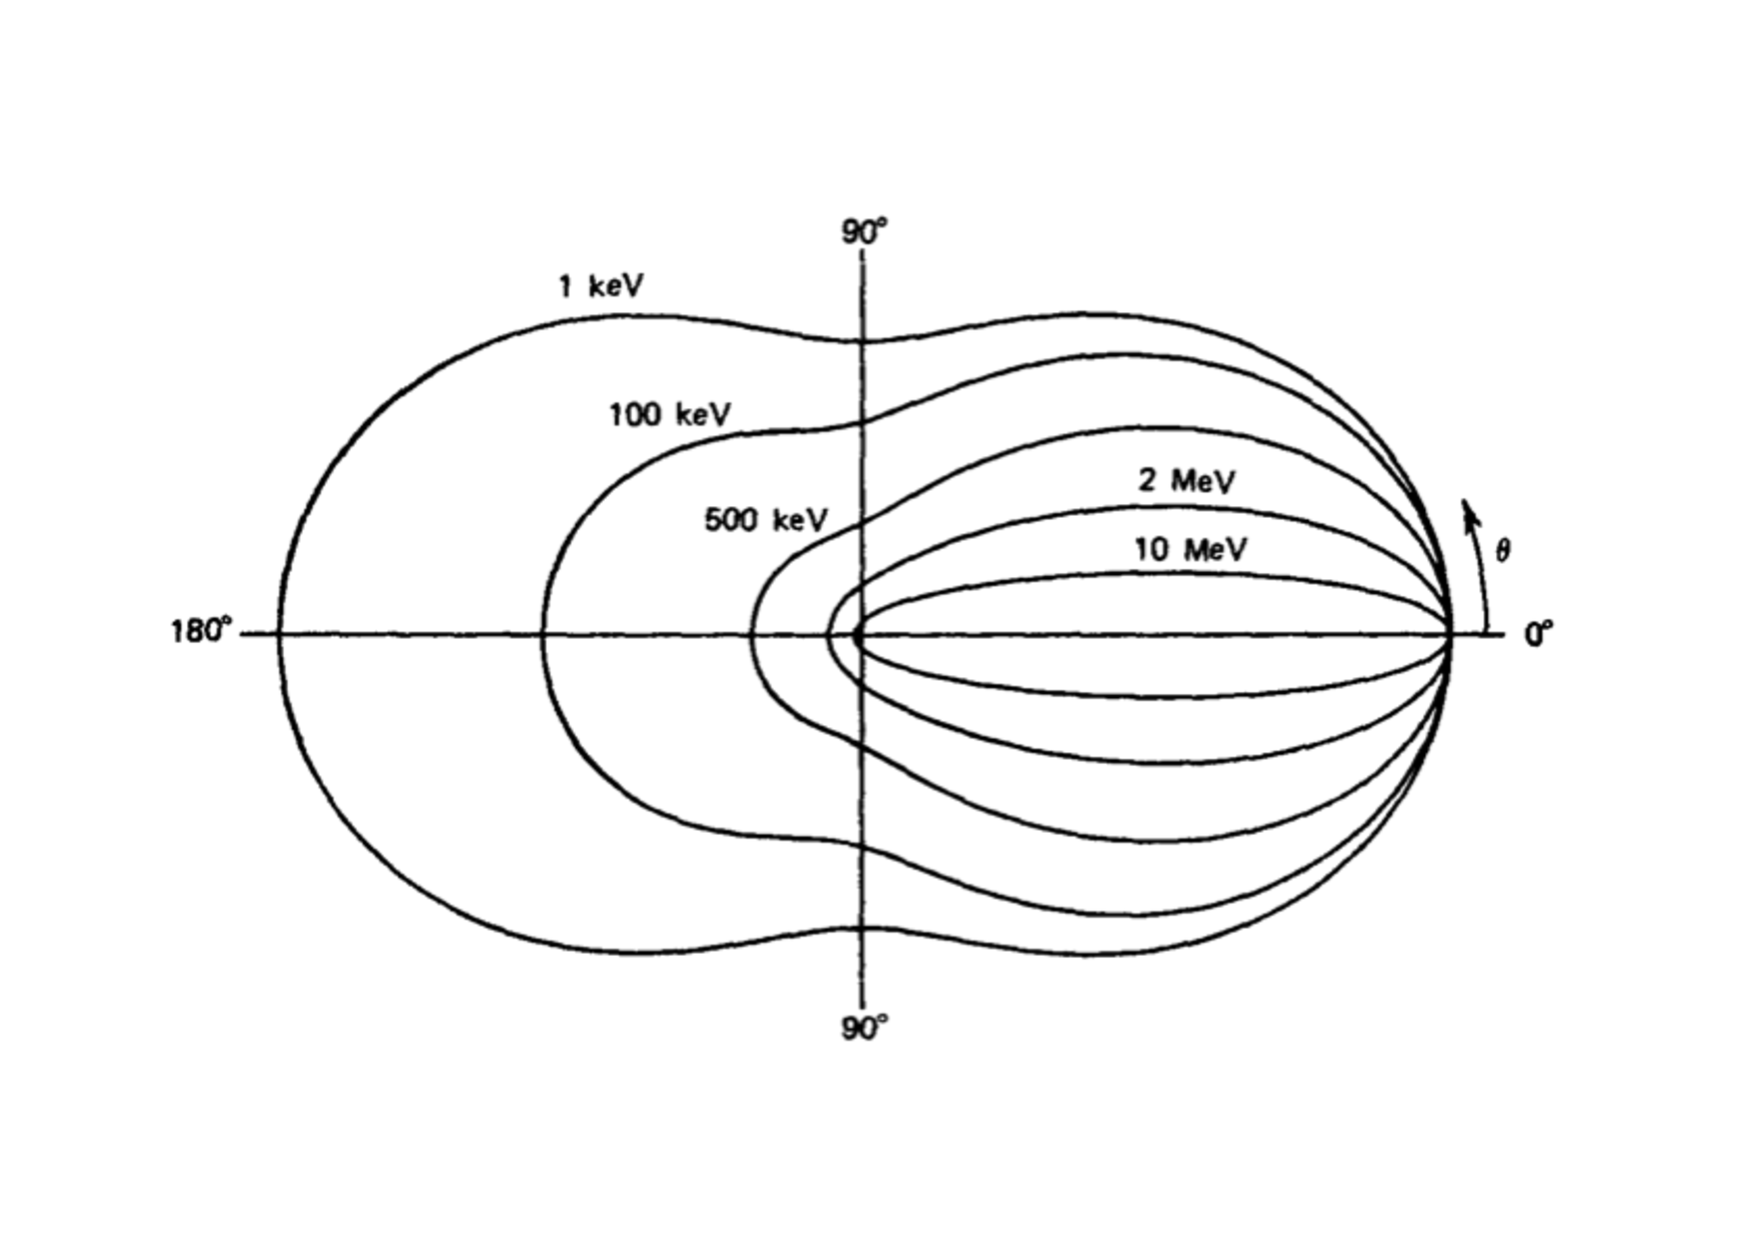
\includegraphics[width=0.8\textwidth]{03_GraphicFiles/chapter2_GammaCameras/ComptonPolar.pdf}
\caption{Polar plot of the number of photons (incident from the left side) Compton scattered into a unit solid angle at the scattering angle $\theta$, for the different indicated incident photon energies. In~\cite{Knoll2000}.}
\label{chap2::fig::ComptonAngCrossSection}
\end{figure}
 
As mentioned, the Compton cross section and energy transfer are calculated with the assumption of free electrons, but at very low incident photon energies such an assumption breaks down and the electronic binding energy $E_B$ affects the Compton interaction: the closer is the photon energy $h\nu$ to $E_B$, the larger is the deviation of the atomic cross section from the one calculated with the Klein-Nishina formula. Various theories have been developed to account for electronic binding energy effects and apply corrections on the Compton atomic cross sections~\parencite{Bergstrom1997}. It is worth to notice that for a given absorber Z, the binding energy correction is more significant at lower photon energies, and for a given initial energy $h\nu$, the binding energy correction is more significant at higher atomic number Z. The described binding energy effect is also referred to as \enquote{Doppler broadening}~\parencite{DuMond1928, DuMond1929}. 
   
If the photon incident energy exceeds twice the the rest-mass energy of and electron \myMarginnote{Pair production} $2m_ec^2 = $ 1.02~MeV, the production of an electron-positron pair in conjunction with a complete absorption of the photon becomes energetically possible. In practice, as shown in \figurename~\ref{chap2::fig::photonCrossSec},  the probability of such an interaction mechanism, referred to as pair production, remains very low until the gamma-ray energy approaches several MeV and therefore pair production is predominantly confined to high-energy photons. For $h\nu > 2m_ec^2$, energy and charge can be conserved even if pair production occurs in free space, but the conservation of linear momentum requires the Coulomb field of a collision partner (atomic nucleus or orbital electron). The photon, indeed, possesses momentum excess that is not absorbed by the electron-positron pair, and must be absorbed by the collision partner. When such an extra momentum is absorbed by the atomic nucleus, the recoil energy, as a result of the relatively large nuclear mass, is exceedingly small and the effect is described as the standard pair production: the incident gamma-ray disappears and is replaced by an electron-positron pair. When an orbital electron of the atom picks up the extra momentum, the recoil energy may be significant and determine the ejection of the orbital electron; in this case, the photon is absorbed and three particles leaves the interaction site, two electrons and a positron, in the so-called \enquote{triplet production}. A schematic representation of these two effects is given in \figurename~\ref{chap2::fig::pairprod}.

\begin{figure}[!htbp]
\centering
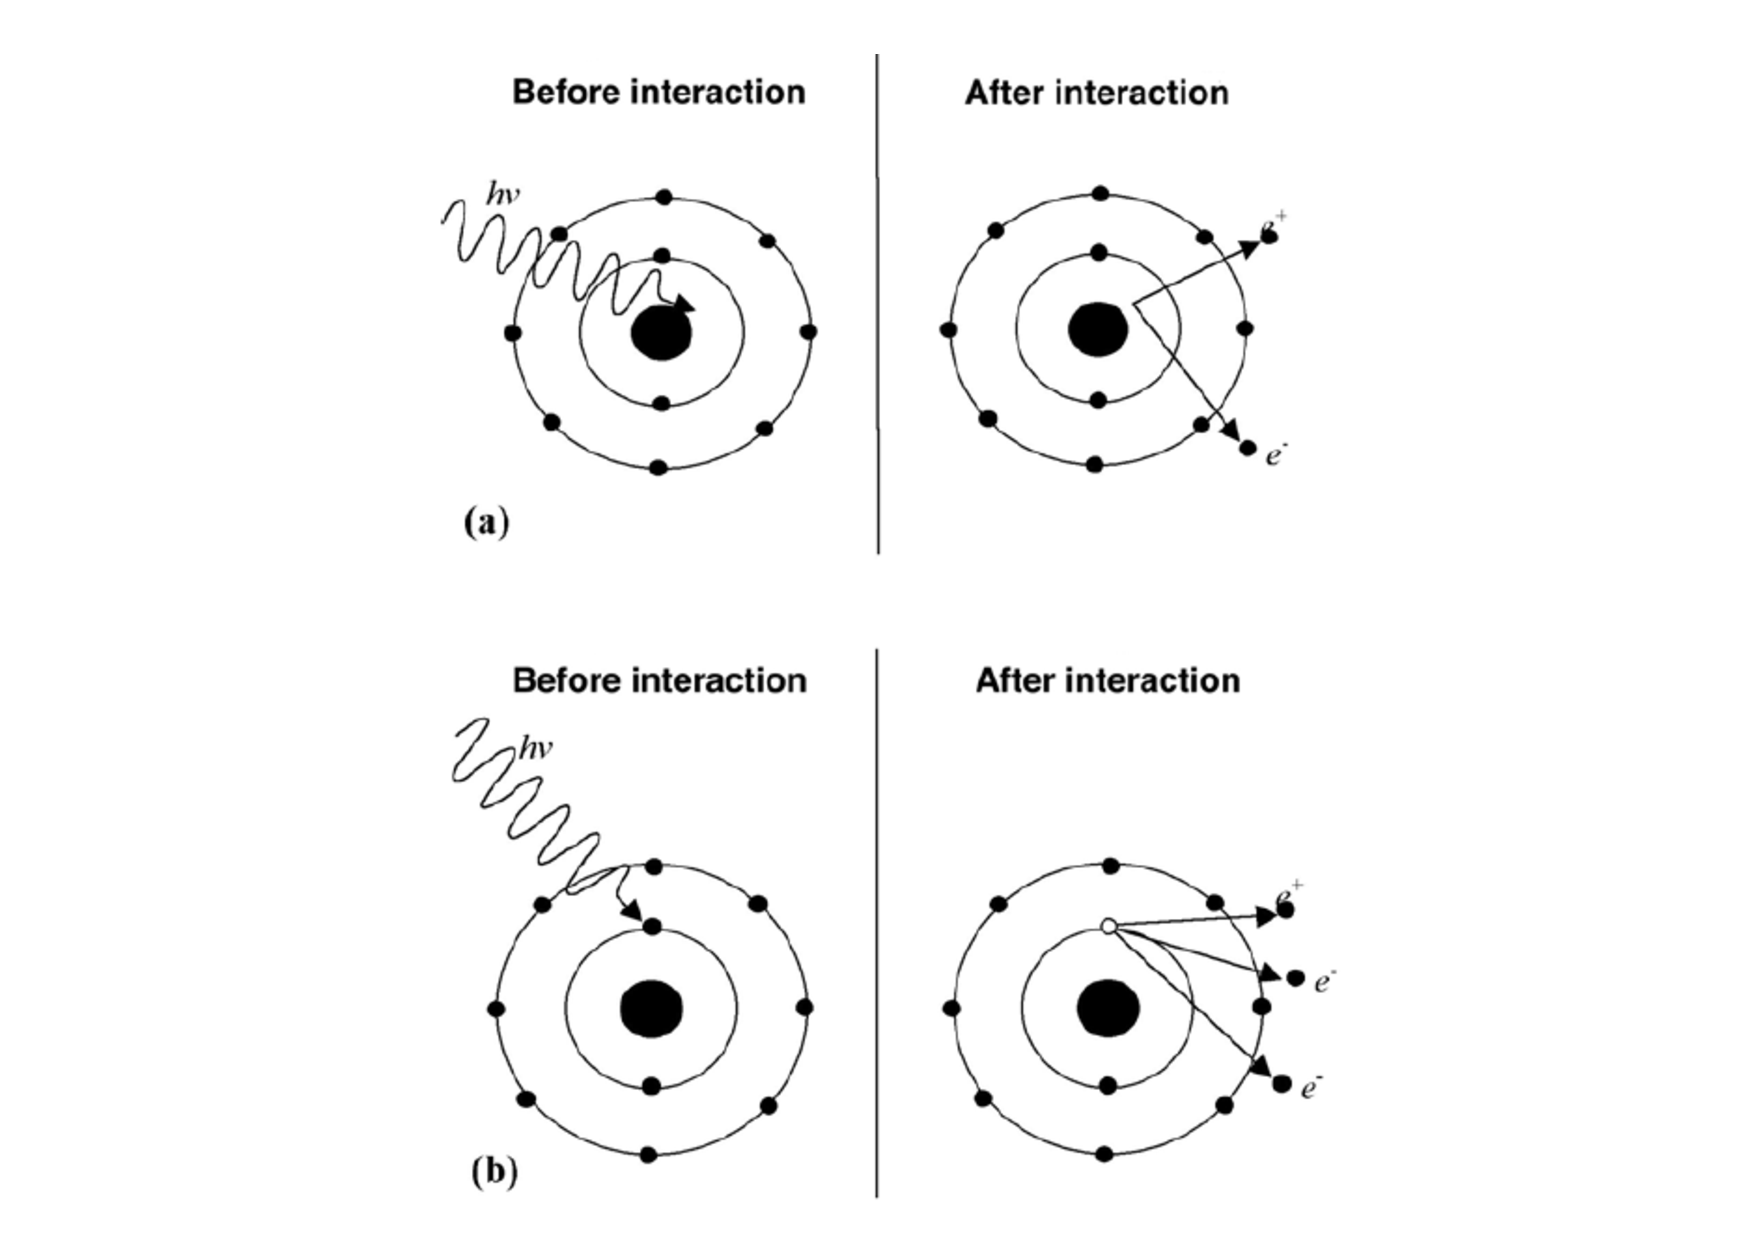
\includegraphics[width=0.9\textwidth]{03_GraphicFiles/chapter2_GammaCameras/pairProd.pdf}
\caption{Schematic representation of pari production (a) in the COulomb field of a nucleus and triplet production (b) in the Coulomb field of an orbital electron. In~\cite{Podgirsak2010}.}
\label{chap2::fig::pairprod}
\end{figure} 

The total kinetic energy transferred to the charged particles is the difference between the photon incident energy and twice the rest-mass energy of the positron-electron pair.
In both cases, because the positron will annihilate after slowing down in the absorbing medium, two annihilation photons are normally produced as secondary products of the interaction. 
No simple expression exists for the probability of pair production per nucleus, but its magnitude varies approximately as the square of the absorber atomic number Z, and it rises sharply with the photon energy. 

\begin{figure}[!htbp]
\centering
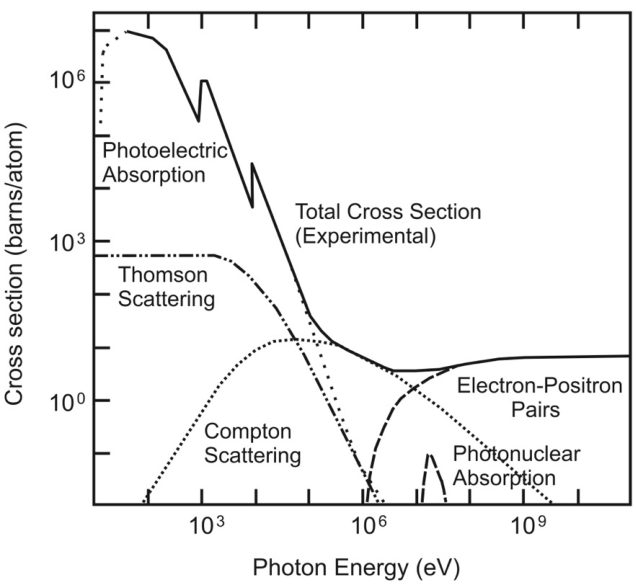
\includegraphics[width=0.8\textwidth]{03_GraphicFiles/chapter2_GammaCameras/Photon-energy-dependent-cross-sections-Cross-sections-of-the-photoelectric-absorption.png}
\caption{Cross sections of the photoelectric absorption, Thomson scattering, Compton scattering, pair production (electron-positron pairs), and photonuclear absorption for a copper absorber as a function
of the photon energy energy. In~\cite{Hermanss2013}.}
\label{chap2::fig::photonCrossSec}
\end{figure} 

The relative importance of the three described interaction processes for different absorber materials (Z) and gamma-ray energies ($h\nu$) are illustrated in \figurename~\ref{chap2::fig::relativePhotonInt}. Three areas are defined by the two solid lines in the plot, which indicates the energy/Z values for which the two neighboring effects have equivalent probability. 
 
\begin{figure}[!htbp]
\centering
\includegraphics[width=0.8\textwidth]{03_GraphicFiles/chapter2_GammaCameras/RelativePhotonInt.pdf}
\caption{Relative importance of the three major types of photon interaction in matter. The lines show the values of Z and $h\nu$ for which the two neighboring effects are just equal. In~\cite{Knoll2000}.}
\label{chap2::fig::relativePhotonInt}
\end{figure} 


If we now consider a photon beam interacting with a target, all the mentioned interaction processes removes gamma-ray photons from the beam either by absorption or by scattering away from the beam direction, and can be characterized by a fixed probability of occurrence per unit path length in the absorber. The sum of these probabilities is simply the probability per unit path length that the photon is lost and is referred to as \enquote{linear attenuation coefficient} $\mu$. Ther number of transmitted photons $I$ can be then expresses in terms of the number of incident photons in the beam $I_0$ as a function of the linear attenuation coefficient and the absorber thickness $t$, as shown by equation~\ref{chap2::eq::attenuation}.

 \begin{equation}
\frac{I}{I_0} = e^{-\mu t}
\label{chap2::eq::attenuation}
\end{equation} 

The average distance traveled by the a photon of the beam in the absorber before an interaction takes place is called \enquote{mean free path} $\lambda$, and is the reciprocal of the linear attenuation coefficient. In solids, for common gamma-ray energies, $\lambda$ can vary in the range between few millimeters to tens of centimeters. 
A more widely used parameter is the \enquote{mass attenuation coefficient} $\mu_{\rho}$, which normalize the linear attenuation coefficient to the absorber density $\rho$ (equation~\ref{chap2::eq::massAttenuation}).

\begin{equation}
\mu_{\rho} = \frac{\mu}{\rho}
\label{chap2::eq::massAttenuation}
\end{equation} 

If the mass attenuation coefficient is used, the convenient concept of mass thickness is also introduced, corresponding to the product of the absorber thickness $t$ by its density $\rho$ and generally measured in mg/cm$^2$. For compound and mixtures, the mass attenuation coefficient is approximated by a summation of a weighted average of its constituent, as expressed in equation~\ref{chap2::eq::massAttCoeffCompoud}.

 \begin{equation}
\mu_{\rho} = \sum_i{w_i\frac{\mu_i}{\rho}}
\label{chap2::eq::massAttenuation}
\end{equation} 

with $w_i$ the proportion by weight of the i-th constituent, and $\mu_i/rho$ its mass attenuation coefficient. The attenuation coefficients have specific values for a given photon energy $h\nu$ and absorber atomic number Z, and are tabulated on the \gls{nist} database according to the calculations in~\cite{Seltzer1993}.

\section{Ion range monitoring with prompt-gamma radiation}

As introduced in chapter~\ref{chap::1}, the high ballistic precision of particle therapy is advantageous because it provides high dose selectivity while sparing the healthy tissues surrounding the tumors, but at the same time it makes such a cancer care modality quite sensitive to any source of uncertainty and deviation with respect to the treatment planning: patient mispositioning, organ motion or anatomical between fractions (such as tumor shrinking, weight loss, cavity filling). A reduction of the safety margins presently applied to the \gls{ptv} to account for such uncertainties would be only possible with the availability of a real-time range monitoring system. As the primary beam stops inside the patient, the range control should be based on secondary radiations issued from nuclear reactions. In particular, the work presented in this thesis is focused on range monitoring techniques relying on the detection of \gls{pg} rays.
 
\section{\gls{pg} emission during particle therapy}

The \gls{pg} range monitoring techniques rely on the emission of photons due to the de-excitation of excited nuclei within about one nanosecond after the nuclear interaction. The \glspl{pg} are emitted in the whole solid angle around the patient and in a wide energy range (from some hundreds of keV up to 10 MeV). 

\begin{figure}
\centering
\begin{subfigure}[t]{.49\textwidth}
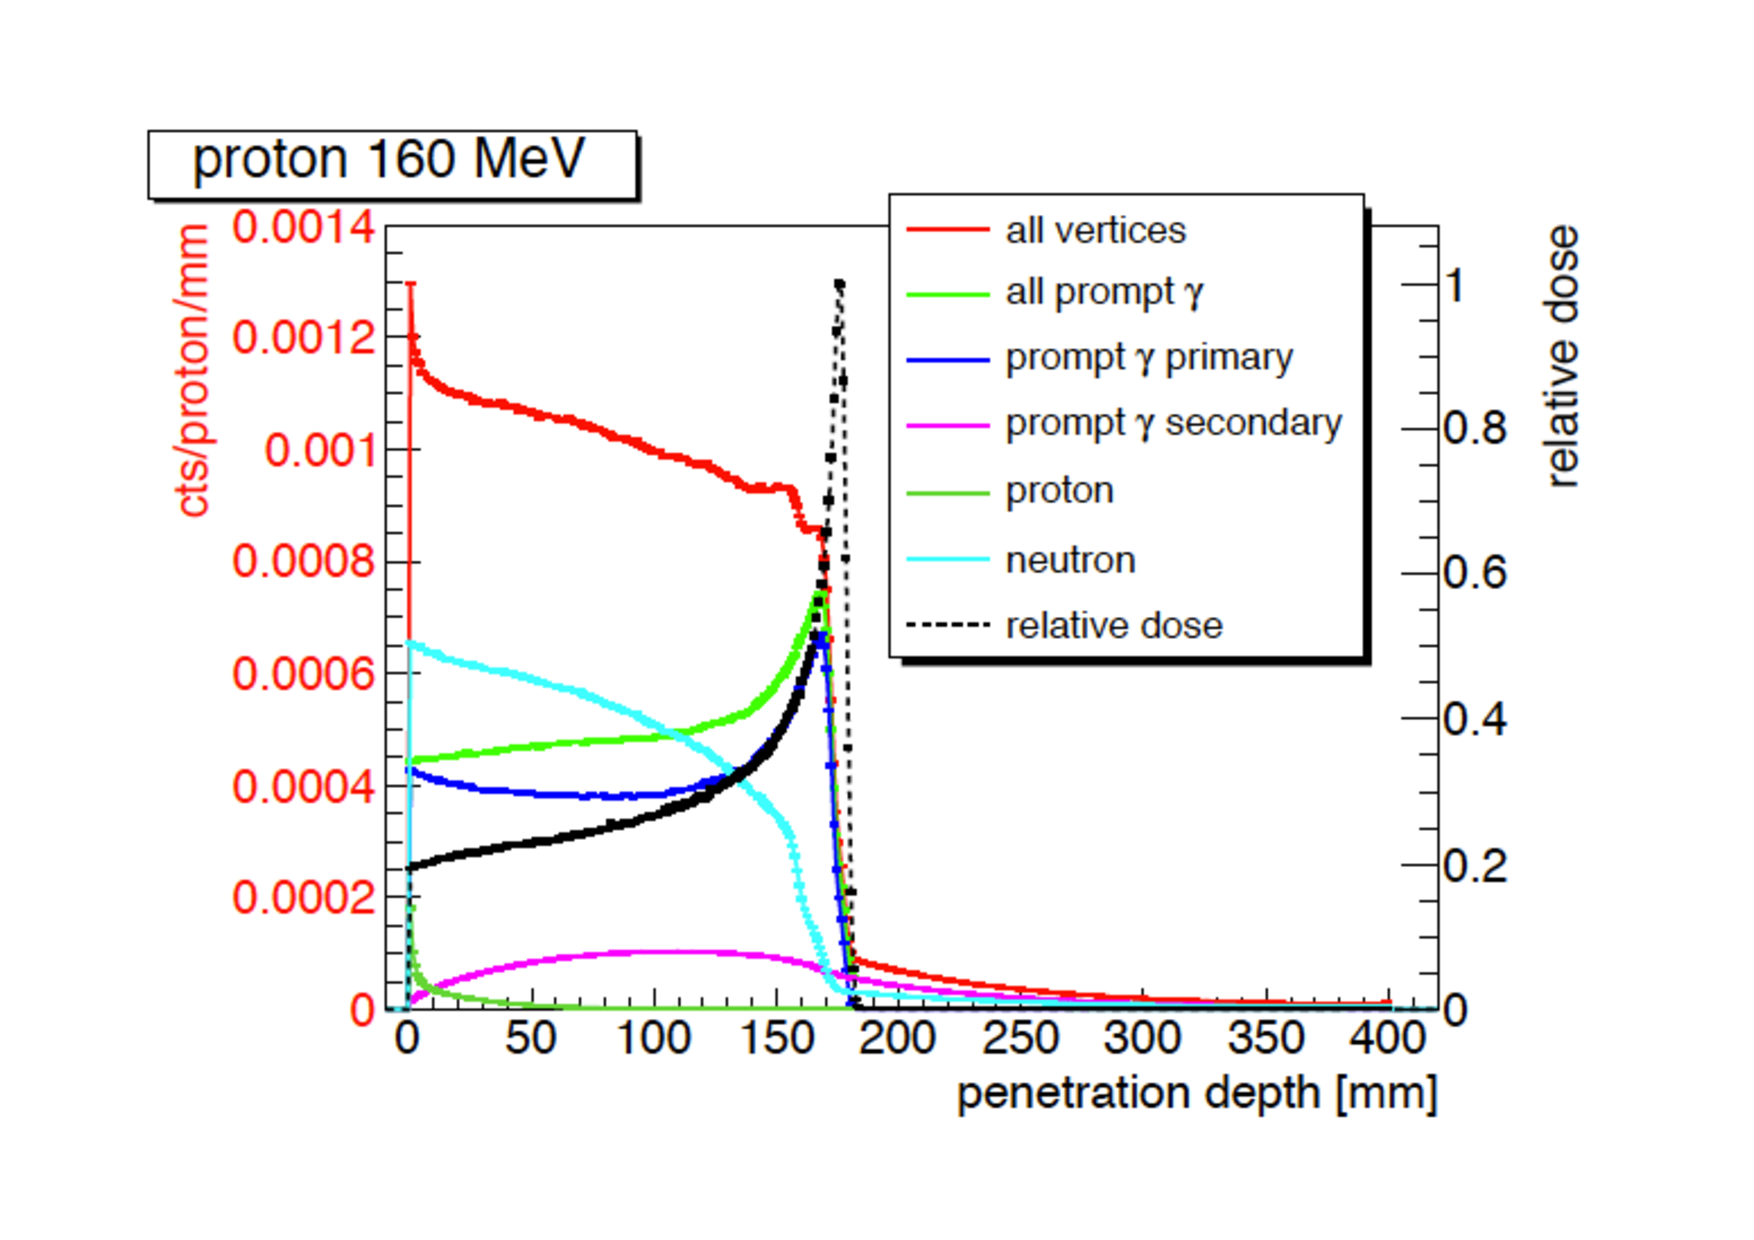
\includegraphics[width=1.2\linewidth]{03_GraphicFiles/chapter2_GammaCameras/PG_secPartDistr_p.pdf}
\caption{Emission vertices of secondary particles emerging from a cylindrical water target (15~cm diameter, 40~cm length) irradiated by a 160~MeV proton beam. An energy lower threshold of 1~MeV has been applied.}
\label{chap2::fig::PGsecDistrp}
\end{subfigure}
\begin{subfigure}[t]{.49\textwidth}
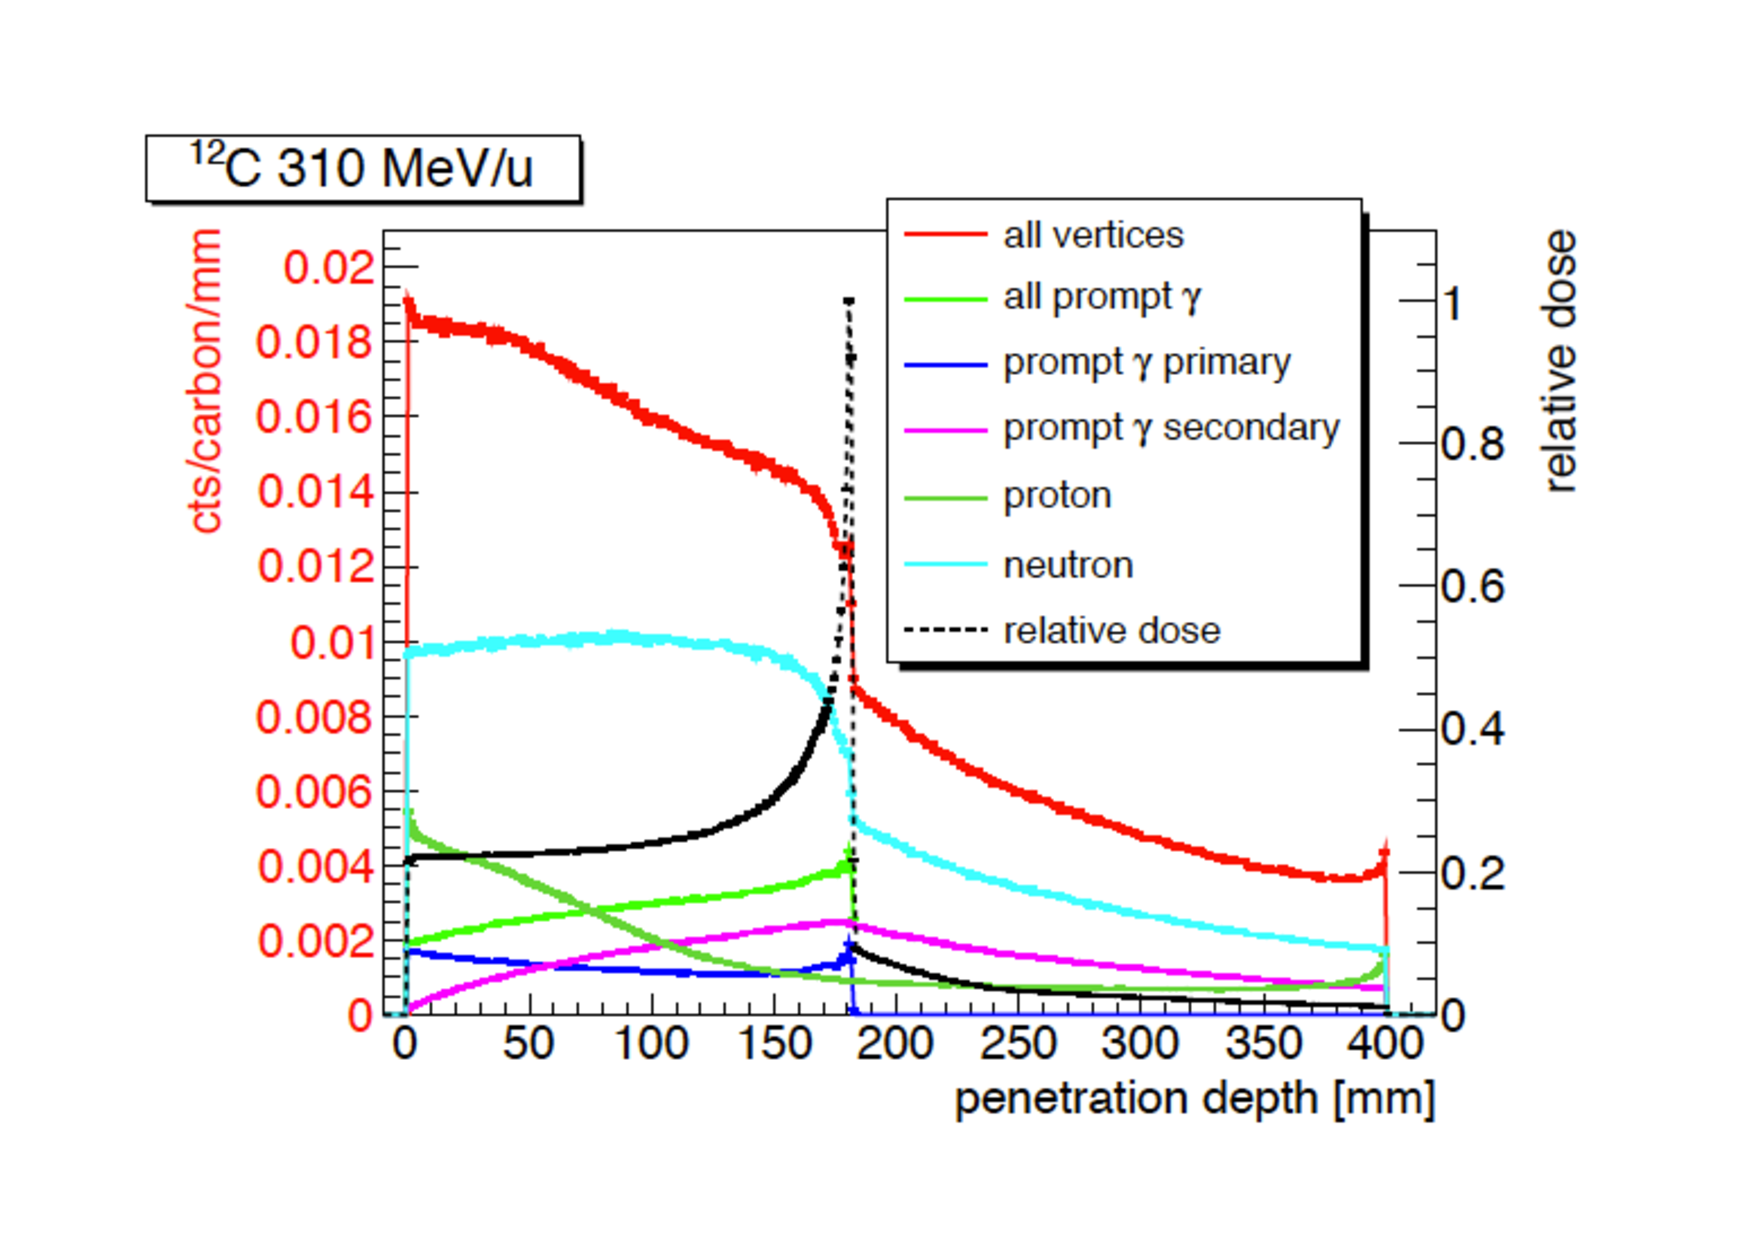
\includegraphics[width=1.2\linewidth]{03_GraphicFiles/chapter2_GammaCameras/PG_secPartDistr_C.pdf}
\caption{Emission vertices of secondary particles emerging from a cylindrical water target (15~cm diameter, 40~cm length) irradiated by a 310~MeV/u carbon ion beam. An energy lower threshold of 1~MeV has been applied.}
\label{chap2::fig::PGsecDistrC}
\end{subfigure}
\caption{In~\cite{Krimmer2017}.}
\label{chap2::fig::PGsecDistr_gen}
\end{figure}


Such a prompt radiation has been demonstrated to be correlated to the ion range for both protons and carbon ions. It can be exploited via single photon detection systems to provide a real-time feedback in case of major deviations of the measured range with respect to the planned one, and eventually trigger a treatment emergency stop.

LINE CONE RECONSTRUCTION \parencite{Cree1994}, \parencite{Basko1998}, \parencite{Parra1999}, \parencite{Hirasawa2003}, \parencite{Maxim2009} 

ITERATIVE RECONSTRUCTION \parencite{Schone2010}, \parencite{Zoglauer2011}, \parencite{Gillam2011}, \parencite{Lojacono2013}, \parencite{Mackin2012}


\section{Gamma cameras state of the art}

\clearpage
%\printbibliography[heading=subbibintoc]
